\documentclass[varwidth, border=0pt]{standalone}

\usepackage{times}      % Loads the Times-Roman Fonts
\usepackage{mathptmx}   % Loads the Times-Roman Math Fonts
\usepackage{subcaption}
\usepackage[labelfont={bf,sf},%
labelsep=period,%
justification=centering,
labelformat=parens,labelsep=quad,skip=3pt,font=scriptsize]{caption}
\usepackage{graphicx}

\begin{document}
	
\begin{figure}[H]
	\centering
	\begin{subfigure}{0.5\linewidth}
		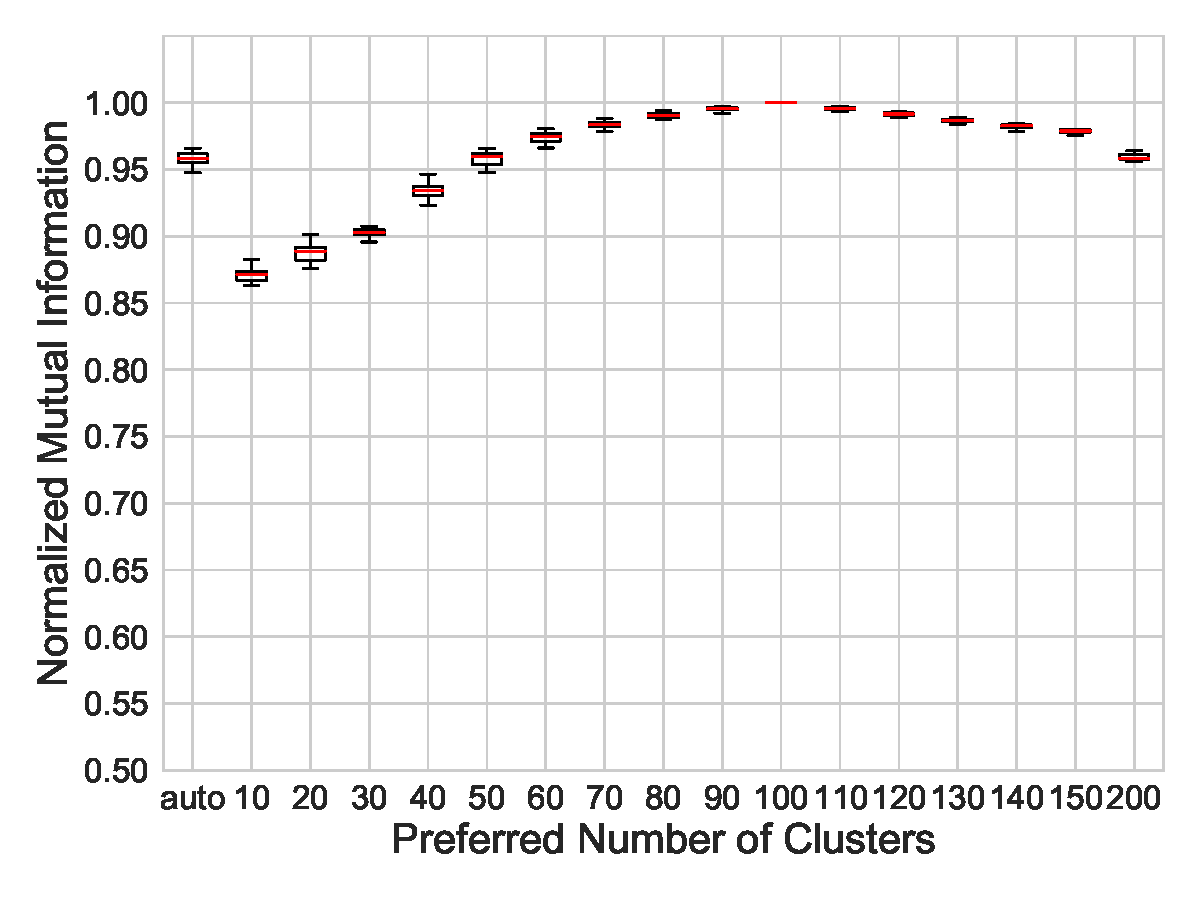
\includegraphics[width=\linewidth]{../../graphics/preferred_number_of_modules_nmi_us}
		\subcaption{United States (Normalized Mutual Information)}
	\end{subfigure}~%
	\begin{subfigure}{0.5\linewidth}
		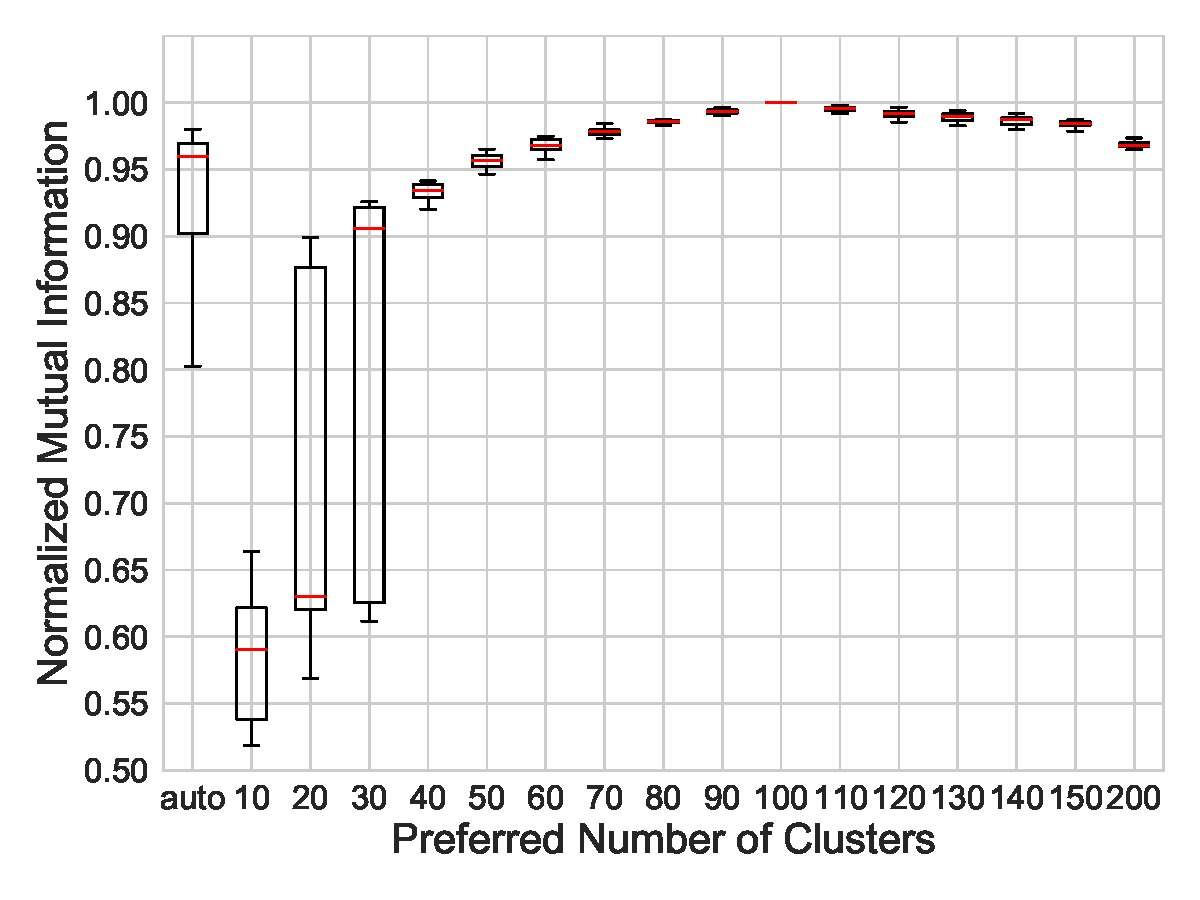
\includegraphics[width=\linewidth]{../../graphics/preferred_number_of_modules_nmi_de}
		\subcaption{Germany (Normalized Mutual Information)}
	\end{subfigure}
	\begin{subfigure}{0.5\linewidth}
		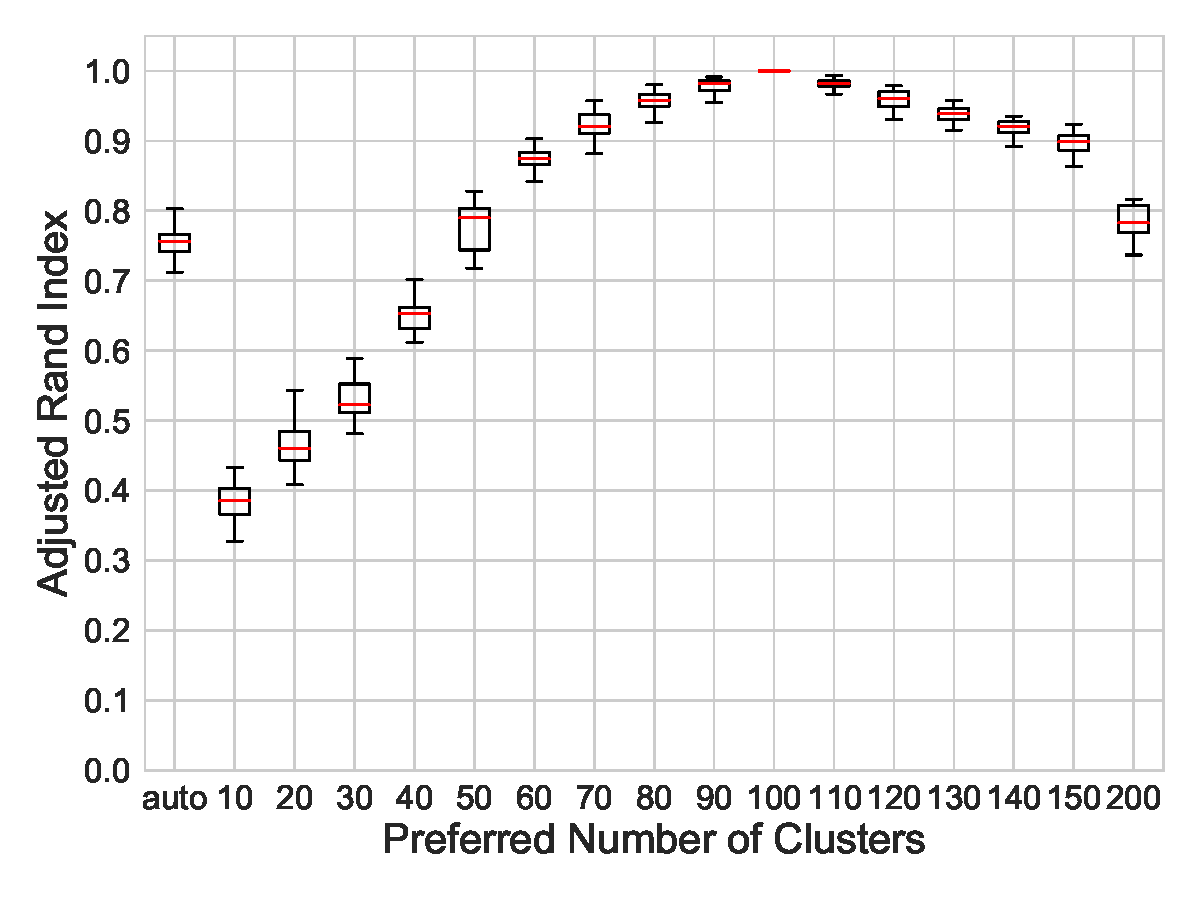
\includegraphics[width=\linewidth]{../../graphics/preferred_number_of_modules_rand_us}
		\subcaption{United States (Adjusted Rand Index)}
	\end{subfigure}~%
	\begin{subfigure}{0.5\linewidth}
		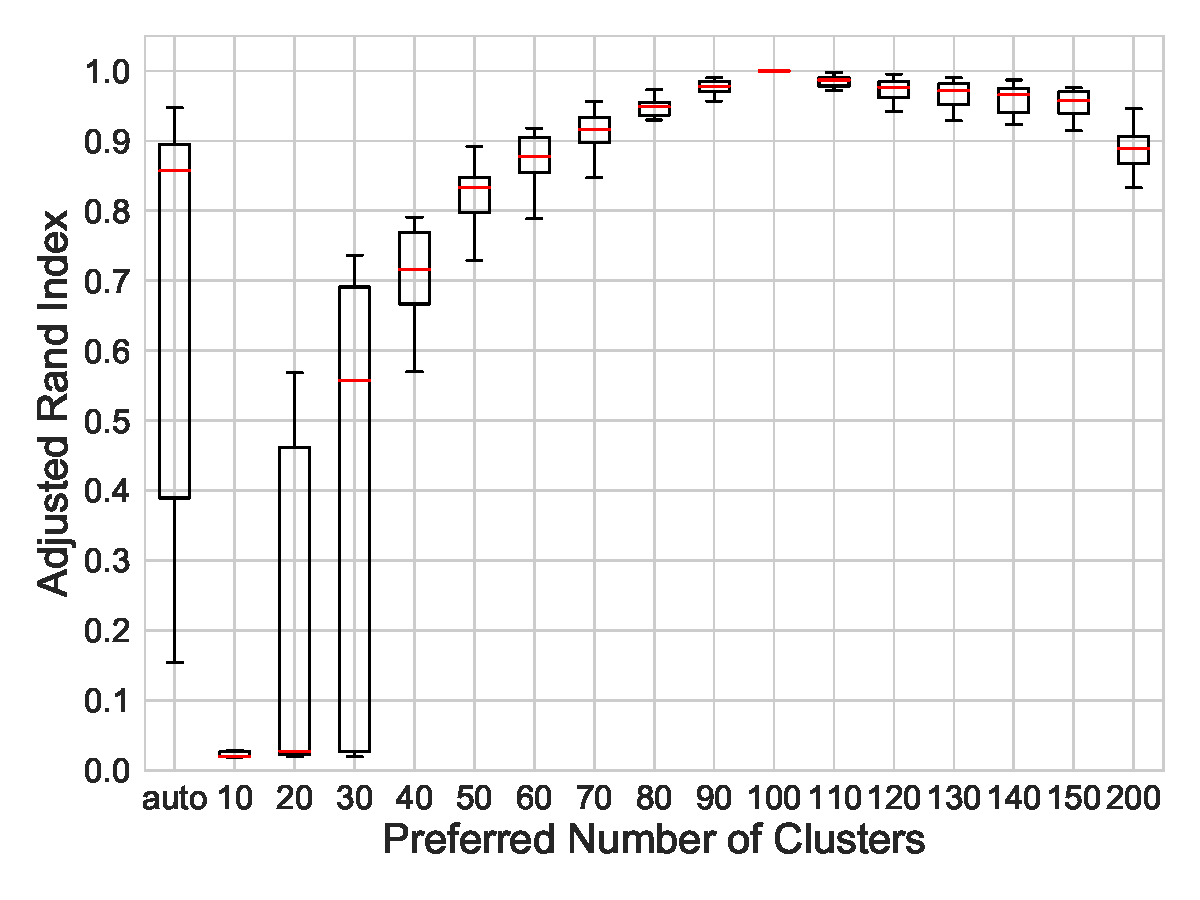
\includegraphics[width=\linewidth]{../../graphics/preferred_number_of_modules_rand_de}
		\subcaption{Germany (Adjusted Rand Index)}
	\end{subfigure}

\end{figure}
	
\end{document}
